\begin{His}

Au lieu de se demander quels nombres sont solutions d'une équation donnée, on peut considérer le problème inverse : de quelles équations un nombre donné est-il solution ? Un nombre est dit \textit{rationnel} s'il est solution d'une équation du premier degré à coefficients entiers. Il est dit \textit{algébrique} s'il est solution d'une équation polynomiale à coefficients entiers. S'il n'est pas algébrique il est dit \textit{transcendant}. Ainsi, pour un nombre donné, l'objectif est de trouver les éventuelles équations polynomiales dont ce nombre est racine.

\vspace{0.4cm}

%Par exemple pour $\sqrt{2}$, la question se pose de savoir s'il est possible de construire une équation du premier degré ayant cette valeur pour racine. Elle se résout simplement : si une telle équation existe, on en déduit l'expression $2a^2 = b^2$, où $a$ et $b$ sont des nombres entiers. L'analyse de la décomposition en facteurs premiers montre que le terme de droite contient le facteur 2 un nombre pair de fois et celui de gauche un nombre impair. Cette remarque démontre que $\sqrt{2}$ n'est pas un nombre rationnel. En revanche, il est par définition algébrique, car solution de l'équation $X^2-2 = 0$.

%\vspace{0.4cm}
%
%La même question pour le nombre $\pi$ est plus délicate. Pour montrer que ce nombre n'est solution d'aucune équation du premier degré à coefficients dans les nombres entiers, on utilise des fractions continues généralisées (une démonstration est proposée dans l'article « Fraction continue et approximation diophantienne »). Les techniques sont plus sophistiquées que celles utilisées pour démontrer l'irrationalité de $\sqrt{2}$. Alors que ce premier résultat est déjà connu à l'époque d'Euclide, il faut attendre le XVIIIe siècle pour établir celle de $\pi$.

\vspace{0.4cm}
\begin{wrapfigure}[10]{r}{3.6cm}
\vspace{-7mm}
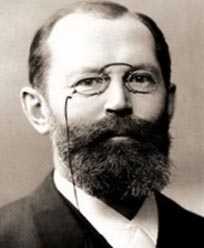
\includegraphics[scale=0.5]{image_chapitres/lindemann.jpg} 
\unnumberedcaption{C. L. F. von \textsc{Lindemann}}
\end{wrapfigure}
Si montrer que $\pi$ n'est pas solution d'une équation du premier degré à coefficients dans les entiers n'est déjà pas si simple, il est encore plus ardu de montrer qu'il n'est solution d'aucune équation polynomiale à coefficients entiers. Il faut encore plus d'un siècle d'efforts pour établir cette transcendance. Elle clôt une vieille question, à savoir s'il est possible de construire à la règle et au compas un carré de même aire qu'un cercle, cette question porte le nom de \textit{quadrature du cercle}. Elle est impossible car toute construction de cette nature définit une surface d'aire égale à un nombre algébrique.
\vspace{0.4cm}

\textbf{Carl Louis Ferdinand \textsc{von Lindemann}} (12 avril 1852 à Hanovre - 6 mars 1939 à Munich) est un mathématicien allemand. Il est passé à la postérité pour sa démonstration, publiée en 1882, de la transcendance du nombre $\pi$, c'est-à-dire qu'il n'existe aucun polynôme non nul à coefficients rationnels dont $\pi$ soit une racine.


\PESP{https://fr.wikipedia.org/wiki/Équation}

\end{His}
